\documentclass[12pt]{report}\usepackage[]{graphicx}\usepackage[dvipsnames]{xcolor}
% maxwidth is the original width if it is less than linewidth
% otherwise use linewidth (to make sure the graphics do not exceed the margin)
\makeatletter
\def\maxwidth{ %
  \ifdim\Gin@nat@width>\linewidth
    \linewidth
  \else
    \Gin@nat@width
  \fi
}
\makeatother

\definecolor{fgcolor}{rgb}{0.345, 0.345, 0.345}
\newcommand{\hlnum}[1]{\textcolor[rgb]{0.686,0.059,0.569}{#1}}%
\newcommand{\hlstr}[1]{\textcolor[rgb]{0.192,0.494,0.8}{#1}}%
\newcommand{\hlcom}[1]{\textcolor[rgb]{0.678,0.584,0.686}{\textit{#1}}}%
\newcommand{\hlopt}[1]{\textcolor[rgb]{0,0,0}{#1}}%
\newcommand{\hlstd}[1]{\textcolor[rgb]{0.345,0.345,0.345}{#1}}%
\newcommand{\hlkwa}[1]{\textcolor[rgb]{0.161,0.373,0.58}{\textbf{#1}}}%
\newcommand{\hlkwb}[1]{\textcolor[rgb]{0.69,0.353,0.396}{#1}}%
\newcommand{\hlkwc}[1]{\textcolor[rgb]{0.333,0.667,0.333}{#1}}%
\newcommand{\hlkwd}[1]{\textcolor[rgb]{0.737,0.353,0.396}{\textbf{#1}}}%
\let\hlipl\hlkwb

\usepackage{framed}
\makeatletter
\newenvironment{kframe}{%
 \def\at@end@of@kframe{}%
 \ifinner\ifhmode%
  \def\at@end@of@kframe{\end{minipage}}%
  \begin{minipage}{\columnwidth}%
 \fi\fi%
 \def\FrameCommand##1{\hskip\@totalleftmargin \hskip-\fboxsep
 \colorbox{shadecolor}{##1}\hskip-\fboxsep
     % There is no \\@totalrightmargin, so:
     \hskip-\linewidth \hskip-\@totalleftmargin \hskip\columnwidth}%
 \MakeFramed {\advance\hsize-\width
   \@totalleftmargin\z@ \linewidth\hsize
   \@setminipage}}%
 {\par\unskip\endMakeFramed%
 \at@end@of@kframe}
\makeatother

\definecolor{shadecolor}{rgb}{.97, .97, .97}
\definecolor{messagecolor}{rgb}{0, 0, 0}
\definecolor{warningcolor}{rgb}{1, 0, 1}
\definecolor{errorcolor}{rgb}{1, 0, 0}
\newenvironment{knitrout}{}{} % an empty environment to be redefined in TeX

\usepackage{alltt}

\usepackage[utf8]{inputenc}
\usepackage[spanish]{babel}
\usepackage[margin=2.54cm]{geometry}
\usepackage[dvipsnames]{xcolor}
\usepackage{array, amssymb, amsthm, enumitem, fancyhdr, float, graphicx, mathtools, hyperref}

\pagestyle{fancy}
\lhead{\footnotesize \leftmark}
\rhead{\footnotesize \rightmark}

\title{
	\huge
	\noindent\textbf{Fundamentos de la Ciencia de Datos}\\
	
	{\Large \textit{Práctica 1}}
	\vspace{1cm}
	
	\huge
	Grado en Ingeniería Informática\\
	Universidad de Alcalá\\
	
	\vspace{1cm}
	
	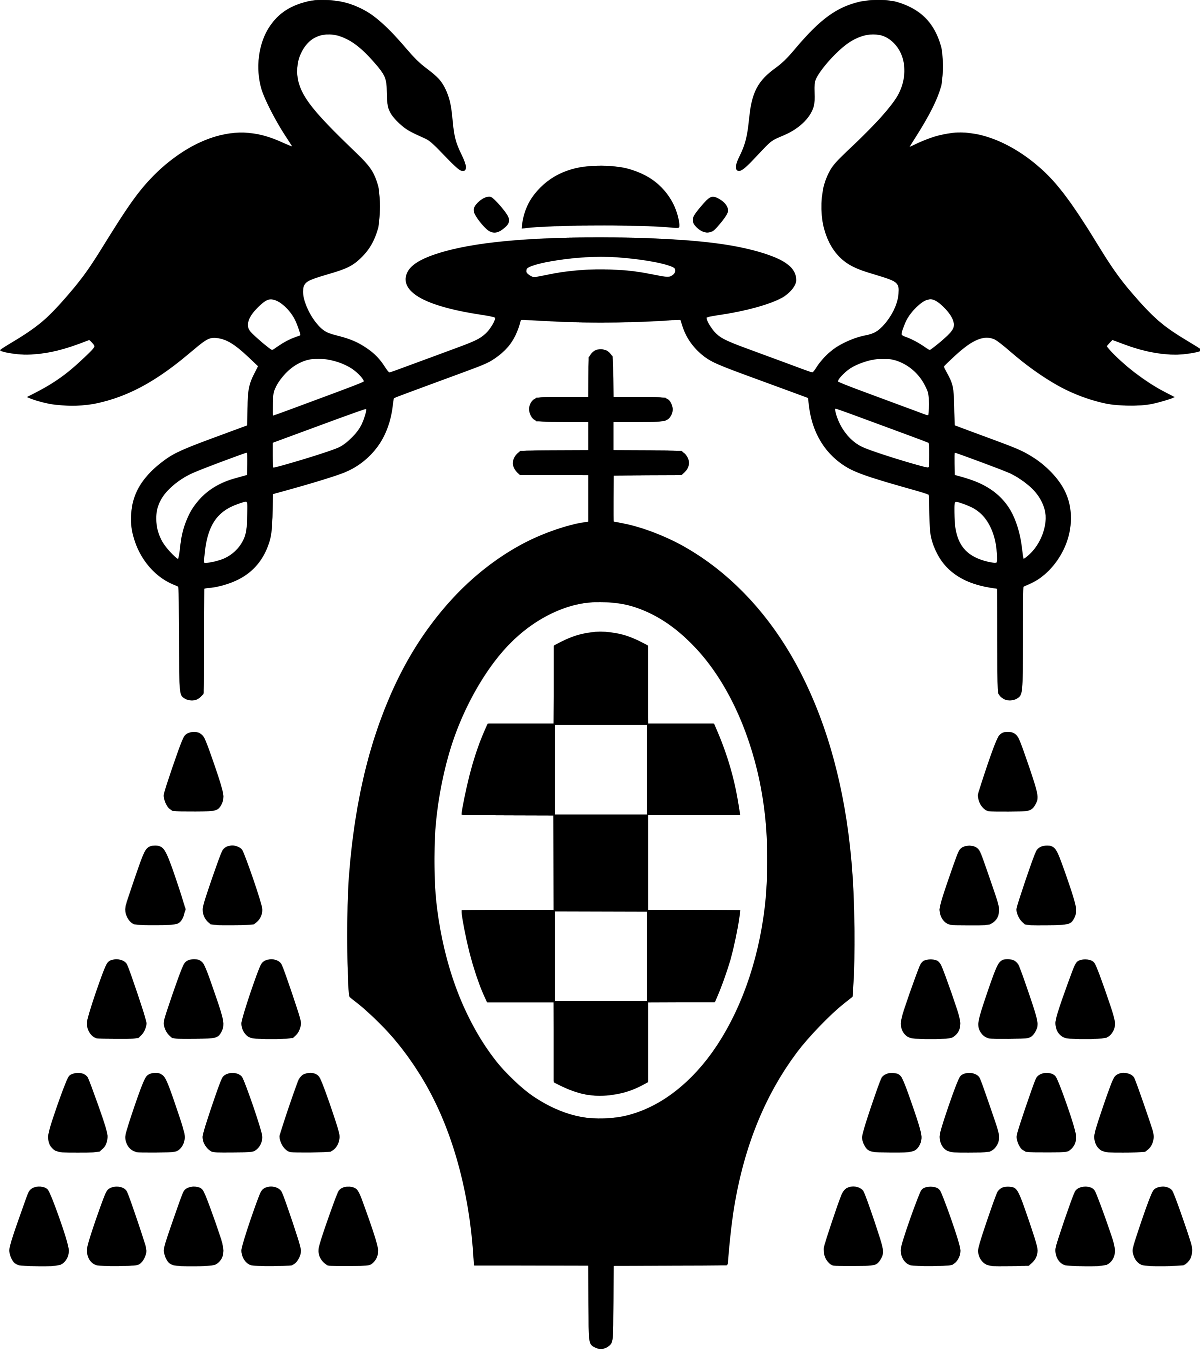
\includegraphics[scale=0.075]{img/logo}
}

\author{
	Pablo García García\\
	Abel López Martínez\\
	Álvaro Jesús Martínez Parra\\
	Raúl Moratilla Núñez
}

\date{
	\large{14 de noviembre de 2023}
}

\hypersetup{
	pdftitle={Práctica 1}, 
	pdfauthor={Pablo García García, Abel López Martínez, Álvaro Jesús Martínez Parra, Raúl Moratilla Núñez}, 
	pdfsubject={Fundamentos de la Ciencia de Datos}, 
	pdfcenterwindow, 
	pdfnewwindow=true, 
	pdfkeywords={Entrega de la PL1 de laboratorio correspondiente al Curso 2023-2024}, 
	bookmarksopen=true 
}
\IfFileExists{upquote.sty}{\usepackage{upquote}}{}
\begin{document}
	
	\renewcommand{\tablename}{Tabla}
	\renewcommand{\chaptername}{Parte}
	\maketitle \thispagestyle{empty}
	
	\newpage
	
	\tableofcontents
	
	\chapter*{Introducción}
	
	\chapter{Ejercicios guiados}
	
		En esta primera parte de esta práctica, repetirán los ejercicios explicados y realizados por el profesor en las clases de laboratorio, utilizando los mismos procedimientos vistos plasmándolos en un documento \LaTeX{}. 
	
		\section{Descripción de los datos}
		
			``\textit{El primer conjunto de datos, que se empleará para realizar el análisis de descripción de datos, estará formado por datos de una característica cualitativa, nombre, y otra cuantitativa, radio, de los satélites menores de Urano, es decir, aquellos que tienen un radio menor de 50 Km, dichos datos, los primeros cualitativos nominales, y los segundos cuantitativos continuos, son: (Nombre, radio en Km): Cordelia, 13; Ofelia, 16; Bianca, 22; Crésida, 33; Desdémona, 29; Julieta, 42; Rosalinda, 27; Belinda, 34; Luna-1986U10, 20; Calíbano, 30; Luna-999U1, 20; Luna 1999U2, 15.}''\\
			
			Para comenzar con la resolución de este ejercicio, deberemos escribir los datos en un fichero \texttt{.txt}, cumpliendo las siguientes normas: 
			
			\begin{itemize}
				\item Existirá una tabulación entre dato y dato. 
				\item La primera columna numera las filas, y en la primera fila se introduce un espacio y el nombre de las variables. 
				\item Se introducirá un salto de línea en la última fila
				\item Para los números decimales se utilizarán puntos. 
				\item Al escribir nombres, no se deberán introducir espacios. 
			\end{itemize}
			
			Obedeciendo a estas normas, copiamos los datos en un fichero llamado \texttt{satelites.txt}, y lo cargamos en R de la siguiente manera: 
			
\begin{knitrout}
\definecolor{shadecolor}{rgb}{0.969, 0.969, 0.969}\color{fgcolor}\begin{kframe}
\begin{alltt}
\hlstd{s} \hlkwb{<-} \hlkwd{read.table}\hlstd{(}\hlstr{"data/satelites.txt"}\hlstd{)}
\hlkwd{print}\hlstd{(s)}
\end{alltt}
\begin{verbatim}
##          nombre radio
## 1      Cordelia    13
## 2        Ofelia    16
## 3        Bianca    22
## 4       Crésida    33
## 5     Desdémona    29
## 6       Julieta    42
## 7     Rosalinda    27
## 8       Belinda    34
## 9  Luna-1986U10    20
## 10     Calíbano    30
## 11   Luna-999U1    20
## 12  Luna-1999U2    15
\end{verbatim}
\end{kframe}
\end{knitrout}
			
			Ahora en la variable \texttt{s} tenemos un dataframe con los datos de nuestros satélites. En los dataframes se accede por \texttt{[fila, columna]}, y también podemos consultar las dimensiones con la función \texttt{dim}. Sería de esperar que nos dijera que tiene 12 filas (los 12 datos), y 2 columnas (\texttt{nombre} y \texttt{radio}). 
			
\begin{knitrout}
\definecolor{shadecolor}{rgb}{0.969, 0.969, 0.969}\color{fgcolor}\begin{kframe}
\begin{alltt}
\hlkwd{dim}\hlstd{(s)}
\end{alltt}
\begin{verbatim}
## [1] 12  2
\end{verbatim}
\end{kframe}
\end{knitrout}
			
			También podemos ordenar el dataframe, en función de una de las magnitudes (columnas), usando la función \texttt{order} aplicando recursivamente el concepto de acceder por filas y columnas. Veamos un ejemplo, si en \texttt{s} teníamos guardado nuestro dataframe, y queremos ordenar por \texttt{radio}, la manera de hacerlo sería la siguiente: 
			
\begin{knitrout}
\definecolor{shadecolor}{rgb}{0.969, 0.969, 0.969}\color{fgcolor}\begin{kframe}
\begin{alltt}
\hlstd{s_ordered} \hlkwb{<-} \hlstd{s[}\hlkwd{order}\hlstd{(s}\hlopt{$}\hlstd{radio), ]}
\hlkwd{print}\hlstd{(s_ordered)}
\end{alltt}
\begin{verbatim}
##          nombre radio
## 1      Cordelia    13
## 12  Luna-1999U2    15
## 2        Ofelia    16
## 9  Luna-1986U10    20
## 11   Luna-999U1    20
## 3        Bianca    22
## 7     Rosalinda    27
## 5     Desdémona    29
## 10     Calíbano    30
## 4       Crésida    33
## 8       Belinda    34
## 6       Julieta    42
\end{verbatim}
\end{kframe}
\end{knitrout}
			
			Podemos introducir nuevos criterios a la ordenación, como por ejemplo, hacerlo en orden descendente. Para esto usaremos la función \texttt{rev}. 
			
\begin{knitrout}
\definecolor{shadecolor}{rgb}{0.969, 0.969, 0.969}\color{fgcolor}\begin{kframe}
\begin{alltt}
\hlstd{s_ordered_rev} \hlkwb{<-} \hlstd{s[}\hlkwd{rev}\hlstd{(}\hlkwd{order}\hlstd{(s}\hlopt{$}\hlstd{radio)), ]}
\hlkwd{print}\hlstd{(s_ordered_rev)}
\end{alltt}
\begin{verbatim}
##          nombre radio
## 6       Julieta    42
## 8       Belinda    34
## 4       Crésida    33
## 10     Calíbano    30
## 5     Desdémona    29
## 7     Rosalinda    27
## 3        Bianca    22
## 11   Luna-999U1    20
## 9  Luna-1986U10    20
## 2        Ofelia    16
## 12  Luna-1999U2    15
## 1      Cordelia    13
\end{verbatim}
\end{kframe}
\end{knitrout}
		
		\section{Asociación}
		
			``\textit{El segundo conjunto de datos, que se empleará para realizar el análisis de asociación, estará formado por las siguientes 6 cestas de la compra: \{Pan, Agua, Leche, Naranjas\}, \{Pan, Agua, Café, Leche\}, \{Pan, Agua, Leche\}, \{Pan, Café, Leche\}, \{Pan, Agua\}, \{Leche\}.}''
		
		\section{Detección de datos anómalos}
		
			\subsection{Primer ejercicio}
			
				``\textit{El tercer conjunto de datos, que se empleará para realizar el análisis de detección de datos anómalos utilizando técnicas con base estadística, estará formado por los siguientes 7 valores de resistencia y densidad para diferentes tipos de hormigón \{Resistencia, Densidad\}: \{3, 2; 3.5, 12; 4.7, 4.1; 5.2, 4.9; 7.1, 6.1; 6.2, 5.2; 14, 5.3\}. Aplicar las medidas de ordenación a la resistencia y las de dispersión a la densidad.}''
			
			\subsection{Segundo ejercicio}
			
				``\textit{El cuarto conjunto de datos, que se empleará para realizar el análisis de detección de datos anómalos utilizando técnicas basadas en la proximidad y en la densidad, estará formado por las siguientes 5 calificaciones de estudiantes: 1. \{4, 4\}; 2. \{4, 3\}; 3. \{5, 5\}; 4. \{1, 1\}; 5. \{5, 4\} donde las características de las calificaciones son: (Teoría, Laboratorio).}''
	
	\chapter{Ejercicios autónomos}
	
		\section{Descripción de los datos}
		
			``\textit{El primer conjunto de datos, que se empleará para realizar el análisis de descripción de datos, estará formado por datos de una característica cuantitativa, distancia, desde el domicilio de cada estudiantes hasta la Universidad, dichos datos, cuantitativos continuos, son: 16.5, 34.8, 20.7, 6.2, 4.4, 3.4, 24, 24, 32, 30, 33, 27, 15, 9.4, 2.1, 34, 24, 12, 4.4, 28, 31.4, 21.6, 3.1, 4.5, 5.1, 4, 3.2, 25, 4.5, 20, 34, 12, 12, 12, 12, 5, 19, 30, 5.5, 38, 25, 3.7, 9, 30, 13, 30, 30, 26, 30, 30, 1, 26, 22, 10, 9.7, 11, 24.1, 33, 17.2, 27, 24, 27, 21, 28, 30, 4, 46, 29, 3.7, 2.7, 8.1, 19, 16.}''
		
		\section{Asociación}
		
			``\textit{El segundo conjunto de datos, que se empleará para realizar el análisis de asociación, estará formado por las siguientes conjuntos de extras incluidos en 8 ventas de coches: \{X, C, N, B\}, \{X, T, B, C\}, \{N, C, X\}, \{N, T, X, B\}, \{X, C, B\}, \{N\}, \{X, B, C\}, \{T, A\}. Donde: \{X: Faros de Xenon, A: Alarma, T: Techo Solar, N: Navegador, B: Bluetooth, C: Control de Velocidad\}, son los extras que se pueden incluir en cada coche.}''
		
		\section{Detección de datos anómalos}
		
			\subsection{Primer ejercicio}
			
				``\textit{El tercer conjunto de datos, que se empleará para realizar el análisis de detección de datos anómalos utilizando técnicas con base estadística, estará formado por los siguientes 10 valores de velocidades de respuesta y temperaturas normalizadas de un microprocesador \{Velocidad, Temperatura\}: \{10, 7.46; 8, 6.77; 13, 12.74; 9, 7.11; 11, 7.81; 14, 8.84; 6, 6.08; 4, 5.39; 12, 8.15; 7, 6.42; 5, 5.73\}. Aplicar las medidas de ordenación a la velocidad y las de dispersión a la temperatura.}''
			
			\subsection{Segundo ejercicio}
			
				``\textit{El cuarto conjunto de datos, que se empleará para realizar el análisis de detección de datos anómalos utilizando técnicas basadas en la proximidad y en la densidad, estará formado por el número de Mujeres y Hombres inscritos en una serie de cinco seminarios que se han impartido sobre biología. Los datos son: \{Mujeres, Hombres\}: 1. \{9, 9\}; 2. \{9, 7\}; 3. \{11, 11\}; 4. \{2, 1\}; 5. \{11, 9\}.}''
	
\end{document}          
